\section{Problemática}

%---------------------------------------------------------

\begin{frame}
	\frametitle{Problemática}
	\begin{itemize}
		\item <1-> Conocer la situación de uso actual de suelo de un punto de interés requiere dinero y tiempo (ir directamente)
		\item <2-> Incongruencias con información brindada por entidades del estado 
		\item <3-> El monitoreo de áreas cultivadas se vuelve tedioso y requiere de mayor inversión en personal
		\item <4-> Desconocimiento de influencias sobre el uso de suelo (Fenómeno del Niño y condiciones del ambiente)
		\item <5-> Base débil para toma de decisiones
	\end{itemize}
\end{frame}

%---------------------------------------------------------

\begin{frame}
	\frametitle{La Teledetección de nuestro lado}
	\textbf{Beneficios:}
	
	\begin{itemize}
		\item Adquisición de información espacial y temporal sobre un objeto de interés sin tener contacto directo con el mismo y de manera sencilla
		\item Poder analizar información difícilmente apreciable por el ojo humano (Espectro Electromagnético)
	\end{itemize}
	
	\begin{figure}
		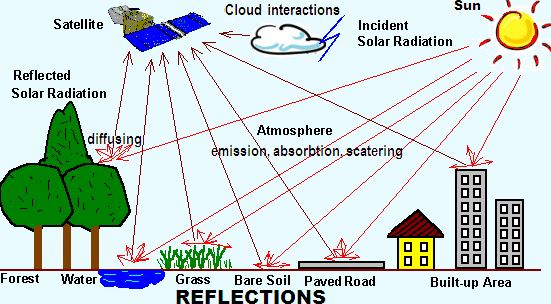
\includegraphics[scale=0.45]{imgs/remote_sensing.JPG}\
		\centering
	\end{figure}
	
\end{frame}

%---------------------------------------------------------

\begin{frame}{La Teledetección de nuestro lado}
	\textbf{Limitaciones:}
	\begin{itemize}
		\item <1-> Diferenciar un cultivo de otro es complicado
		\begin{itemize}
			\item Elevación
			\item Propiedad del suelo
			\item Temperatura
			\item Humedad
			\item Fertilización
			\item Sistema de irrigación
			\item Fecha de plantación
			\item Técnicas y Operación del cultivo
		\end{itemize}
		\item <2-> Similitud en reflectancia y variaciones espaciales, espectrales relacionados a la fenología del cultivo
		\item <3-> Método no fácil de interpretar y operar 
	\end{itemize}
\end{frame}

%---------------------------------------------------------

\begin{frame}
	\frametitle{Artículo Científico}
	
	\begin{figure}
		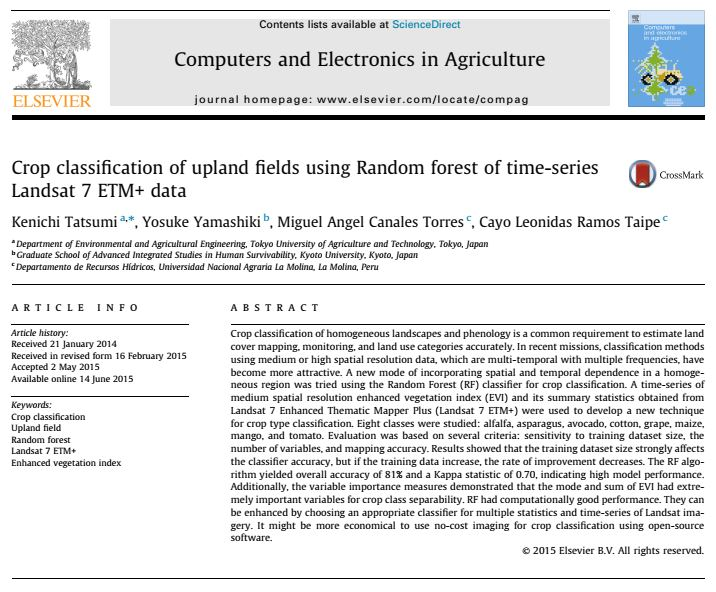
\includegraphics[scale=0.4]{imgs/paper.JPG}\\
		\footnotesize{http://dx.doi.org/10.1016/j.compag.2015.05.001}
		\centering
	\end{figure}
\end{frame}